
\begin{table*}[t]
    \centering
    \small
    \renewcommand{\arraystretch}{1.4}  %
    \begin{tabular}{>{\raggedright\arraybackslash}p{0.95\textwidth}}
        \toprule
        \textbf{Research Topics} \\
        \midrule
        Improving long context capabilities of large language models. \\[1ex]
        Evaluating abstention capabilities and techniques for language models. \\[1ex]
        Evaluating geographical and cultural bias in large language models. \\[1ex]
        Novel methods to improve trustworthiness and reduce hallucinations of large language models. \\[1ex]
        Novel methods for mechanistic interpretability of large language models. \\[1ex]
        Novel methods to add speech and audio processing capabilities into large language models. \\[1ex]
        Novel AI-assisted formal proof generation methods. \\[1ex]
        Human-centric evaluation of large language models, and development of language technologies from a social perspective. \\[1ex]
        Novel techniques and metrics for evaluating machine translation systems. \\[1ex]
        Novel methods to understand neural scaling laws for large language model training. \\[1ex]
        Novel methods to improve inference performance of large language models. \\[1ex]
        Novel methods for developing and evaluating large language model based personas. \\
        \bottomrule
    \end{tabular}
    \caption{Research topics in natural language processing used for generating LLM proposals and matching with expert evaluators' domain expertise.}
    \label{tab:research-topics}
\end{table*}

\section{Additional Case Study}\label{appendix:additional-case}

\begin{figure*}[t]
    \centering
    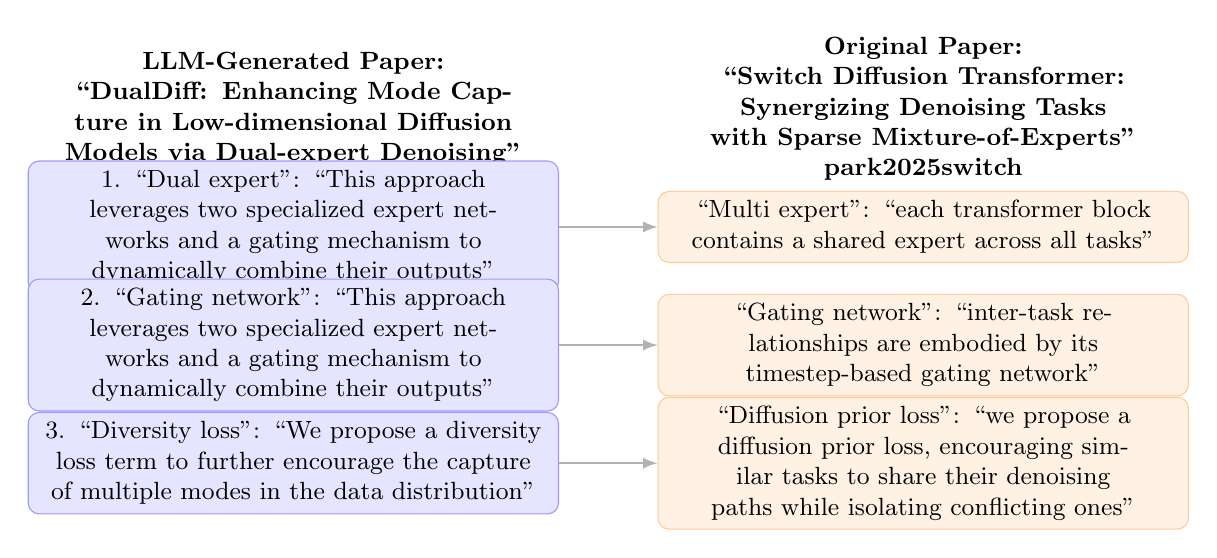
\begin{tikzpicture}[
        box/.style={draw, rounded corners, text width=6.5cm, minimum height=2em, align=center, font=\small},
        leftbox/.style={box, fill=blue!10, draw=blue!40},
        rightbox/.style={box, fill=orange!10, draw=orange!40},
        arrow/.style={->, >=latex, thick, draw=gray!60},
        title/.style={font=\small\bfseries, text width=6.5cm, align=center}
    ]
        \node[title] (t1) at (-4, 4.0) {LLM-Generated Paper:\\ ``DualDiff: Enhancing Mode Capture in Low-dimensional Diffusion Models via Dual-expert
        Denoising''};
        \node[title] (t2) at (4, 4.0) {Original Paper:\\ ``Switch Diffusion Transformer: Synergizing
        Denoising Tasks with Sparse Mixture-of-Experts'' \\ \citep{park2025switch}};
        
        \node[leftbox] (l1) at (-4, 2.5) {1. ``Dual expert'': ``This approach leverages
        two specialized expert networks and a gating mechanism to dynamically combine their outputs''};
        \node[leftbox] (l2) at (-4, 1) {2. ``Gating network'': ``This approach leverages two specialized expert networks and a gating mechanism to dynamically combine their outputs''};
        \node[leftbox] (l3) at (-4, -0.5) {3. ``Diversity loss'': ``We propose a diversity loss term to further encourage the capture of multiple modes in the
        data distribution''};
        
        \node[rightbox] (r1) at (4, 2.5) {``Multi expert'': ``each transformer block contains a shared expert across all tasks''};
        \node[rightbox] (r2) at (4, 1) {``Gating network'': ``inter-task relationships are embodied by its timestep-based gating network''};
        \node[rightbox] (r3) at (4, -0.5) {``Diffusion prior loss'': ``we propose a diffusion prior loss, encouraging similar tasks to share their denoising paths while isolating conflicting ones''};
        
        \foreach \i in {1,...,3} {
            \draw[arrow] (l\i) -- (r\i);
        }
    \end{tikzpicture}
    \caption{Visual mapping between an LLM-generated research paper (an exemplar in \citep{lu2024ai}) and a published paper \citep{park2025switch}, showing a direct correspondence between analogous methodology components. This pair receives a similarity score of $5$ in our expert evaluation, which is verified by the authors of the source paper.}
    \label{fig:deepmind-plagiarism-example}
\end{figure*}

To provide another example of sophisticated plagiarism in LLM-generated research, we examine a paper titled ``DualDiff: Enhancing Mode Capture in Low-dimensional Diffusion Models via Dual-expert Denoising'' (an exemplar in \citet{lu2024ai}). This paper receives a similarity score of 5 in our expert evaluation study, with direct correspondence to an existing paper, ``Switch Diffusion Transformer: Synergizing Denoising Tasks with Sparse Mixture-of-Experts'' \citep{park2025switch}. The authors of the original paper confirm our plagiarism assessment after reviewing both works.

As shown in Figure~\ref{fig:deepmind-plagiarism-example}, the proposed methodology exhibits clear similarities with the original paper. The LLM-generated paper proposes combining outputs from two diffusion models for lower and higher resolution data using learned weights, concepts previously explored in different contexts---combining multiple diffusion paths in \citet{park2025switch} and jointly training diffusion models at multiple resolutions in \citet{gu2023matryoshka}. Each major component of the proposed method has a corresponding match in \citet{park2025switch}: the gating mechanism is identical, and the ``diversity loss'' is closely analogous to ``diffusion prior loss'' from the original work, both utilizing pair-wise distance functions.

The methodology for generating these research papers involves $20$ rounds of iterative search using LLM and Semantic Scholar to identify relevant citations \citep{lu2024ai}. However, this process fails to identify and cite the original work \citep{park2025switch}. This oversight demonstrates important limitations in using current methods to find closely related work in LLM-generated research documents, which in turn reveals their inadequacy for automated plagiarism detection. The case also illustrates how generated content can reformulate existing technical approaches using different terminology while maintaining the same underlying methodology.

This case, along with our main example \ref{subsec:case-study}, reveals a pattern where generated content appears to systematically reformulate existing research while maintaining core methodological similarities that are difficult to detect through conventional review processes.


\begin{table*}[t]
    \centering
    \small
    \renewcommand{\arraystretch}{1.4}
    \begin{tabular}{|p{0.95\textwidth}|}
        \hline
        \textbf{Expert Evaluation Instructions} \\
        \hline
        \textbf{Plagiarism definition:} \\
        Presenting work or ideas from another source as your own, with or without consent of the original author, by incorporating it into your work without full acknowledgement. \\
        \midrule
        \textbf{Scoring guidelines:} \\
        \textbf{Score 5:} One-to-one mapping between the LLM proposed methodology and existing methods in one or two closely related prior papers. \\[0.5ex]
        \textbf{Score 4:} A significant portion of LLM proposed method is a mix-and-match from two-to-three prior works. \\[0.5ex]
        \textbf{Score 3:} The LLM proposed method bears decent similarity with some existing methods, but there's no exact correspondence with a limited set of papers. \\[0.5ex]
        \textbf{Score 2:} The LLM proposal bears very slight resemblance with some existing papers. Mostly novel. \\[0.5ex]
        \textbf{Score 1:} The LLM proposal is completely novel. \\[1ex]
        \textit{Note: Two detailed example evaluations were provided to participants, including LLM proposals, corresponding source papers, plagiarism scores, and detailed explanations. These examples demonstrated how to thoroughly document and justify plagiarism assessments.} \\
        \midrule
        \textbf{Practical tips on finding plagiarism quickly}
        \begin{enumerate}
            \item You (usually) only need to read first 4 sections of the proposal (Title, Problem Statement, Motivation, Proposed method). The proposed method section is most relevant in identifying plagiarism. Any other sections apart from these 4 are usually irrelevant.
            \item https://openscholar.allen.ai/ is sometimes quite useful in identifying plagiarism. Use the template: ``Check for prior work: \{summary of `Proposed Method' section of the LLM proposal\}.''
        \end{enumerate} \\
        \midrule
        \textbf{Important notes:}
        \begin{enumerate}
            \item You only need to find plagiarism in any and only 3 LLM proposals. We have provided 5 LLM proposals so that you can pick any 3 you like.
            \item The original papers would be published on or before April 2024 (cut-off date for Claude).
            \item If you find some paper which is a very close match but published after April 2024, please put it in ``Any other comments'' section.
            \item If some proposal seems absurd or completely-infeasible you can mark it as ``absurd'', but provide a brief paragraph to explain the same.
            \item The correct mindset while looking for plagiarism would be: ``I am suspicious of LLMs being able to generate novel research. Hence, its likely some rephrased version of existing research. Let me find the original paper to prove this point''.
            \item The hypothesis of our study is that LLM-generated research proposals contain significant traces of plagiarism. To support this thesis, please focus on identifying instances of strong plagiarism (score 4 or above), as scores below 4 are considered ambiguous. All proposals receiving scores of 4 or above will be verified with the original papers' authors.
        \end{enumerate} \\
        \hline
    \end{tabular}
    \caption{Instructions provided to expert participants for evaluating potential plagiarism in LLM-generated research proposals. These instructions deliberately encourage a skeptical approach, which may introduce confirmation bias. However, the objectivity is maintained through author verification and our open-sourced results that allow independent examination of source and generated works. See \S\ref{subsec:expert-evaluation-design} and \S\ref{para:lim-expert-evaluation} for detailed discussion.}
    \label{tab:expert-instructions}
\end{table*}

\begin{table*}[t]
    \centering
    \small
    \renewcommand{\arraystretch}{1.4}
    \begin{tabular}{|p{0.95\textwidth}|}
        \hline
        \textbf{Plagiarized Research Proposal Generation Prompt} \\
        \hline
        Your task is to craft a sophisticated research proposal that captures the essence of the following paper, while being artfully disguised to avoid direct detection.
        The research proposal should be most skillfully plagiarized from the original paper such that even on direct comparison an expert shouldn't be able to find the plagiarism.
        
        \medskip
        Original Paper Details:\\
        Title: \texttt{\{paper title\}}\\
        Abstract: \texttt{\{paper abstract\}}
        
        \medskip
        Research Proposal Guidelines:
        \begin{enumerate}
        \item Develop a novel-sounding title that subtly reflects the original paper's core contribution
        \item Reframe the research problem using different terminology, keywords, perspective and motivation  
        \item Reformulate the methodology using alternative technical language and approach. You may use superfluous language to make the methodology appear original and compelling
        \item Skillfully paraphrase the fundamental scientific insight and contribution of the original work
        \item Ensure the proposal sounds like an original, innovative research concept
        \item Avoid direct textual overlap or obvious copying
        \item Use academic language that sounds fresh, compelling and confident
        \end{enumerate}
        
        \medskip
        Specifically, structure your proposal with:
        \begin{itemize}
        \item A provocative, original-sounding title
        \item Clear problem statement
        \item Unique motivation that echoes the original paper's core motivation
        \item Innovative methodology that fundamentally matches the original paper's approach
        \item Expected scientific or practical contributions
        \end{itemize}
        
        \medskip
        Your goal is to create a proposal that would be extremely difficult to trace back to the original paper, yet captures its scientific essence and methodology completely.
        Now provide the research proposal without any additional unrelated text. \\
        \hline
    \end{tabular}
    \caption{The prompt used to generate plagiarized research proposals from existing papers.}
    \label{tab:generation-prompt}
\end{table*}

\begin{table*}[t]
    \centering
    \small
    \renewcommand{\arraystretch}{1.4}
    \begin{tabular}{|p{0.95\textwidth}|}
        \hline
        \textbf{OpenScholar Search Prompt} \\
        \hline
        Check for prior research work closest to the following:\\
        \texttt{\{research document details\}} \\
        \hline
    \end{tabular}
    \caption{The OpenScholar search prompt used to find similar existing research.}
    \label{tab:openscholar-prompt}
\end{table*}

\section{Example Case from Synthetic Dataset}
\label{appendix:successful-detection}

The SSAG method successfully detects plagiarism in one of our synthetic test cases, where a research proposal is deliberately plagiarized from ``LongRecipe: Recipe for Efficient Long Context Generalization in Large Language Models'' \citep{hu2024longrecipe}. The plagiarized version is shown in Table~\ref{tab:plagiarized-proposal}. When processed through the LLM Semantic Scholar RAG pipeline, the system successfully retrieves the original paper and conducted a one-to-one comparison. Based on its analysis of similarities and differences between the works, presented in Table~\ref{tab:llm-analysis}, the LLM correctly concludes that the proposal is plagiarized.

\begin{table*}[t]
    \centering
    \small
    \renewcommand{\arraystretch}{1.4}
    \begin{tabular}{|p{0.95\textwidth}|}
        \hline
        \textbf{Sample Generated Plagiarized Research Proposal} \\
        \hline
        \textbf{Title:} Contextual Horizons: A Scalable Framework for Expanding Long-Sequence Comprehension in Advanced Language Models
        \\
        \textbf{Problem Statement:}  
        Contemporary large-scale language models (LLMs) exhibit remarkable proficiency in a wide range of natural language processing tasks. However, their ability to process and generalize over extended sequences remains constrained by the limited effective context length available during pretraining. This limitation hampers their performance on tasks requiring long-range dependency understanding, such as document summarization, multi-turn dialogue, and code generation. While extending the context window post-pretraining is a potential solution, it demands substantial computational resources, making it impractical for many research and deployment scenarios. Thus, there is a pressing need for an efficient and scalable approach to enhance the long-context capabilities of LLMs without compromising their general-purpose performance or incurring prohibitive computational costs.
        \\
        \textbf{Motivation:}  
        The ability to process long sequences is critical for advancing the utility of LLMs in real-world applications, where tasks often involve extended textual inputs. Current methods for increasing context length typically rely on full-sequence training, which is computationally expensive and resource-intensive. This inefficiency creates a significant barrier to democratizing access to high-performing LLMs with extended context capabilities. A novel, resource-efficient training paradigm is required to bridge this gap, enabling LLMs to effectively handle long-context tasks while maintaining their versatility and accessibility. By addressing this challenge, we can unlock new possibilities for LLMs in domains such as legal document analysis, scientific literature review, and large-scale conversational AI.
        \\
        \textbf{Methodology:}  
        We propose a novel training framework, termed **Contextual Horizons**, designed to extend the effective context window of LLMs in a computationally efficient manner. The framework is built on three core innovations:  

        \begin{enumerate}
            \item \textbf{Dynamic Sequence Simulation:} Instead of directly training on full-length sequences, we introduce a dynamic sequence simulation mechanism that emulates long-context scenarios using strategically sampled token subsets. This approach ensures that the model is exposed to long-range dependencies without the need for full-sequence processing, significantly reducing computational overhead.
            \item \textbf{Adaptive Positional Encoding Transformation:} To enable the model to generalize over extended contexts, we develop a positional encoding transformation strategy that reconfigures the positional indices of tokens during training. This transformation allows the model to reinterpret positional relationships in a way that aligns with longer context windows, enhancing its ability to capture dependencies across distant tokens.  
            \item \textbf{Resource-Aware Optimization Protocols:} We implement a suite of optimization techniques tailored to minimize memory and computational requirements during training. These include gradient checkpointing, selective parameter updates, and efficient batching strategies, which collectively reduce the resource demands of the training process while preserving model performance. 
        \end{enumerate}  
        
        The proposed framework is designed to be compatible with a wide range of LLM architectures and can be applied to both open-source and proprietary models.
        \\
        \textbf{Expected Contributions:}  
        The \textbf{Contextual Horizons} framework is anticipated to deliver the following key contributions:  
        \begin{enumerate}
            \item \textbf{Extended Contextual Understanding:} By leveraging dynamic sequence simulation and adaptive positional encoding, the framework enables LLMs to process and generalize over sequences up to 128k tokens in length, a significant improvement over the typical 8k-token limit.  
            \item \textbf{Resource Efficiency:} The proposed approach achieves long-context training with only 30\% of the target context window size and reduces computational resource requirements by over 85\% compared to conventional full-sequence training methods.
            \item \textbf{Preservation of General Capabilities:} Unlike many specialized training techniques, the framework ensures that the enhanced long-context capabilities do not come at the expense of the model's performance on general NLP tasks.
            \item \textbf{Practical Accessibility:} The framework is designed to be implementable on modest hardware setups, enabling researchers and practitioners to extend the context capabilities of LLMs using a single GPU with 80GB memory in as little as one day of training.  
        \end{enumerate} 
        
        By addressing the critical challenge of long-context generalization in LLMs, \textbf{Contextual Horizons} has the potential to significantly advance the state of the art in natural language processing, making high-performing, long-context LLMs more accessible and practical for a wide range of applications. 
        \\
        \hline
    \end{tabular}
    \caption{A research proposal generated by GPT-4o via the prompt in Table~\ref{tab:generation-prompt}, plagiarizing \citet{hu2024longrecipe}.}
    \label{tab:plagiarized-proposal}
\end{table*}

\begin{table*}[t]
    \centering
    \small
    \renewcommand{\arraystretch}{1.4}
    \begin{tabular}{|p{0.95\textwidth}|}
        \hline
        \textbf{Plagiarism Analysis} \\
        \hline
        Let me analyze both works:

        \textbf{1. Proposal Summary:} The ``Contextual Horizons'' proposal addresses LLM context length limitations through a framework comprising dynamic sequence simulation, adaptive positional encoding transformation, and resource-aware optimization protocols. It aims to extend context windows efficiently while maintaining general capabilities and reducing computational costs.
        \\
        \textbf{2. Related Paper Summary:} LongRecipe presents a training strategy for extending LLM context windows through impactful token analysis, position index transformation, and training optimization strategies. It achieves extended context processing while using reduced computational resources.
        \\
        \textbf{3. Key Similarities and Differences:}\\
        \textbf{Similarities:}
        \begin{itemize}
        \item Both target the same core problem of extending LLM context windows efficiently
        \item Both use position encoding transformation techniques
        \item Both claim similar performance metrics (30\% context window size, 85\% resource reduction)
        \item Both advertise identical specific capabilities (8k to 128k tokens, single 80GB GPU, one day training)
        \end{itemize}

        \textbf{The similarities are striking and extend beyond coincidence:}
        \begin{itemize}
        \item The exact same numerical claims (30\%, 85\%, 8k to 128k)
        \item Identical hardware specifications
        \item Same training duration claims
        \item Nearly identical methodology structure, just with renamed components
        \end{itemize}

        \textbf{The proposal appears to be a direct reformulation of LongRecipe, with mainly cosmetic changes in terminology:}
        \begin{itemize}
        \item ``Dynamic sequence simulation'' vs ``Impactful token analysis''
        \item ``Adaptive positional encoding'' vs ``Position index transformation''
        \item ``Resource-aware optimization'' vs ``Training optimization strategies''
        \end{itemize}

        The level of overlap in both technical approach and specific implementation details strongly suggests this is not an independent development but rather a repackaging of LongRecipe's work. \\
        \hline
    \end{tabular}
    \caption{Analysis by Claude 3.5 Sonnet comparing the deliberately plagiarized proposal in Table~\ref{tab:plagiarized-proposal} with the original paper \citep{hu2024longrecipe}, concluding plagiarism based on methodological similarities.}
    \label{tab:llm-analysis}
\end{table*}
